% SAGE Publications / sagej.cls
% Short Report: 4000 words, 2-3 figures, 150-word abstract
\documentclass[Afour,sageh,times]{sagej}

\usepackage{moreverb,url}
\usepackage{amsmath,amssymb}
\usepackage{graphicx}
\usepackage{xr-hyper}
\usepackage[colorlinks,bookmarksopen,bookmarksnumbered,citecolor=red,urlcolor=red]{hyperref}
\externaldocument[sup-]{supplementary_material}

\def\volumeyear{2026}

\begin{document}

\runninghead{Correig-Fraga}

\title{An attractor account of numerosity perception}

\author{Eudald Correig-Fraga\affilnum{1}}

\affiliation{%
\affilnum{1}Innovamat Education, Avinguda de la Generalitat, 217, Sant Cugat del Vallès, Catalonia (Spain)}

\corrauth{Eudald Correig-Fraga}

\email{eudald.correig@innovamat.com}

\begin{abstract}

Numerical cognition is classically split between an exact system for small sets and an approximate one for larger sets. An alternative tradition posits a single, discrete numerosity representation but leaves open how one code could also yield approximate numerosity extraction. We give this latter idea a mechanistic form: integers act as memories on a number line, each an attractor well that widens with magnitude, and a scalar estimate initializes the landscape and is stabilized by pattern completion. Approximation at larger numerosities then emerges as the error of a single discrete code rather than a separate, intrinsically noisy system. Fitted to individual visual-enumeration responses, the model outperforms matched non-attractor and Weber-style alternatives, and its dynamics account for response time through convergence time and residual uncertainty. The discrete-to-approximate transition arises where neighbouring wells cease to be resolvable. An exploratory application to developmental dyscalculia localizes differences in numerical resolution, while the scalar interface yields cross-modal predictions.
\end{abstract}

\keywords{numerical cognition, subitizing, exact number system, attractor dynamics, approximate number system}

\maketitle

%% ====================================================================
\section{Introduction}
%% ====================================================================

%% Background

% There is OTS and ANS, and nothing in between
Humans, like many non-human animals, possess a non-symbolic ability to extract numerical information from the environment and represent the numerosity of sets, a capacity commonly termed the number sense~\citep{dehaene_number_2011,nieder_neuronal_2016}. This ability is typically expressed in two characteristic behavioural regimes: small sets, typically up to three or four items, are apprehended rapidly and with high accuracy, a phenomenon known as subitizing~\citep{kaufman_discrimination_1949, mandler_subitizing_1982}. Beyond this range, responses become slower and less accurate, response variability grows with set size, and discrimination depends primarily on the ratio between numerosities~\citep{feigenson_core_2004,dehaene_number_2011}. The standard two-systems account attributes these regimes to distinct mechanisms: a capacity-limited Object Tracking System (OTS), which individuates a few objects in parallel, and an Approximate Number System (ANS), which represents larger numerosities as noisy analogue magnitudes ~\citep{feigenson_representations_2002,piazza_subitizing_2011}. 

% Model by G&G
An alternative account of the number sense treats both regimes as outputs of a single code for discrete numerosities. Gallistel and Gelman proposed that a non-verbal counting process represents discrete, countable quantities as analogue magnitudes generated by successive increments and arranged on a linear scale~\citep{gallistel_preverbal_1992,gallistel_non-verbal_2000}. These representations exhibit scalar variability: their standard deviation grows in proportion to magnitude, so neighbouring magnitude distributions overlap increasingly at larger values. This provides a route by which one code can support highly accurate small-number judgments while yielding increasingly graded, ratio-dependent errors for larger numerosities, without assigning the two regimes to separate systems~\citep{whalen_nonverbal_1999, cordes_variability_2001}.

% Computational work has shown that it might be only one mechanism
Computational work has developed several single-system explanations of the two behavioural regimes. The central comparison for the present study is the pair of capacity-limited accounts developed by Cheyette, Piantadosi, and colleagues. At a normative level, \citet{cheyette_unified_2020} ask how a system with finite information-processing capacity should encode numerosities under a power-law prior. The resulting bounded-optimal code allocates greater precision to small values and progressively coarser precision to larger ones, producing near-exact small-number performance and Weber-like variability without a change of numerical system. At a more visually explicit level, \citet{cheyette_limited_2024} locate the relevant bottleneck in limits on visuospatial memory, which can generate the characteristic psychophysics of numerosity from visual arrays. An earlier, representationally distinct model by \citet{zorzi_computational_1999} established a related point: numerical size and distance effects can emerge from a linear cumulative code coupled to nonlinear response competition, without assuming logarithmic compression or scalar representational noise. Other models have derived numerical sensitivity from recurrent visual dynamics or learned image-computable representations~\citep{sengupta_visual_2014,stoianov_emergence_2012,testolin_visual_2020}. Together, these accounts show that the two behavioural regimes need not imply two numerical systems, while leaving open whether their common source lies in capacity-limited sensory encoding or in the structure and dynamics of a shared numerical representation.

% This visual mechanisms do not explain the numerical code in non-visual tasks, or accounts of cross-model adaptation (Burr), or accounts of accuity related to math knowledge, or IPS causal studies
These visual accounts treat numerosity as a product of modality-specific sensory processing, whether as a consequence of limited visuospatial capacity or as a quantity extracted from the image. Number, however, behaves as an abstract quantity that is not bound to any one sense. It transfers across modalities, so that adapting to a stream of sounds or touches shifts the apparent numerosity of a visual array~\citep{arrighi_generalized_2014}, its acuity tracks numerical experience, sharpening with formal schooling in otherwise comparable adults~\citep{piazza_education_2013, nys_does_2013}, and it depends causally on parietal cortex, where stimulating the intraparietal sulcus disrupts numerosity while sparing lower-level vision~\citep{cappelletti_rtms_2007, dormal_contribution_2012} and focal damage yields acalculias that extend even to enumerating touches~\citep{ashkenazi_basic_2008, cohen_tactile_2018}. This picture is not uniform: nonsymbolic number stays robust with little formal schooling once memory and symbolic demands are minimized~\citep{frank_number_2008, zebian_differences_2012, pica_exact_2004}, so this dichotomy is still under debate. Together, these findings motivate an architecture in which modality-specific sensory processing feeds a shared numerical representation.

% Alternative account of numerosity coding that is modality agnostic and accounts for both accumulation/summation and neural coding of number
We propose a one-dimensional, Hopfield-inspired energy landscape as this shared numerical stage~\citep{hopfield_neural_1982,ramsauer_hopfield_2021}: each integer is a stored memory represented by a basin that becomes broader and shallower with magnitude. We motivate this coupled change in basin width and depth by the cross-linguistic power-law decline in number-word frequency~\citep{dehaene_cross-linguistic_1992}, so that more frequently encountered numbers form narrow, deep basins, whereas less frequent numbers form broad, shallow ones. A one-dimensional estimate $y_0$ of numerosity, supplied by modality-specific sensory processing, initializes the landscape. Recurrent clean-up then stabilizes this evidence through pattern completion, so that denoising, competition among integer memories, and categorical numerical readout arise from the same dynamics. The attractor therefore models the transformation from noisy numerical evidence to an integer response, while the same dynamics link response time to settling time and residual readout uncertainty.

% This explains the two regimes and models G&G
On this view, a single numerical landscape supports two forms of readout. Where neighbouring integer attractors are sufficiently distinct, pattern completion stabilizes noisy evidence around a categorical value, yielding rapid and highly accurate responses. As magnitude increases, adjacent basins broaden, become shallower, and increasingly overlap, so categorical resolution is progressively lost; the same landscape then produces coarser, ratio-dependent estimates. The transition from resolved to approximate responding is therefore not implemented as a switch between numerical systems, but emerges from the geometry of one representation. The model thus gives mechanistic form to the single-code architecture proposed by Gallistel and Gelman, while adding an explicit representational mechanism: integer-centred attractors embedded in a continuous, noisy state space~\citep{gallistel_preverbal_1992, gallistel_non-verbal_2000}.

% Teaser
We test this account on ${\sim}$53,000 individual responses from the brief-exposure dataset of~\citet{cheyette_unified_2020}, spanning five presentation durations from 40 to 640~ms. It reproduces both the underestimation of larger numerosities and the fall-off of exact accuracy with set size, and outperforms a Weber/ANS baseline and their own bounded-optimal model. Turning on the clean-up dynamics improves the fit without adding parameters, while the attractor's settling time and residual readout uncertainty together predict response times within the exact range. We quantify the loss of resolution using both a width-based discriminability threshold and the fitted landscape's basin topology.

%% ====================================================================
\section{Methods}
%% ====================================================================

We thus consider the problem of how our model maps a noisy perceptual input onto a discrete numerical response. We posit an energy landscape defined over a continuous axis $x$, with attractor wells associated with integer positions (Fig.~\ref{fig:conceptual}a). A sensory estimate $y_0$ of the numerosity, produced by visual processing of a set of objects (albeit could be, in principle, also produced by auditory, or tactile stimuli), provides the initial state $y_0$, which we model as a simple noise model whose parameters are fitted to data. Starting from $x = y_0$, the system evolves by gradient descent on the energy landscape until $x$ settles into a stable well, implementing Hopfield-style pattern completion~\citep{hopfield_neural_1982}. A probability distribution over integers is then read out from the final resting state $x^*$. The same dynamics, combined with an entropy readout that characterizes uncertainty, also determine how long the trial takes.

\begin{figure}[t]
  \centering
  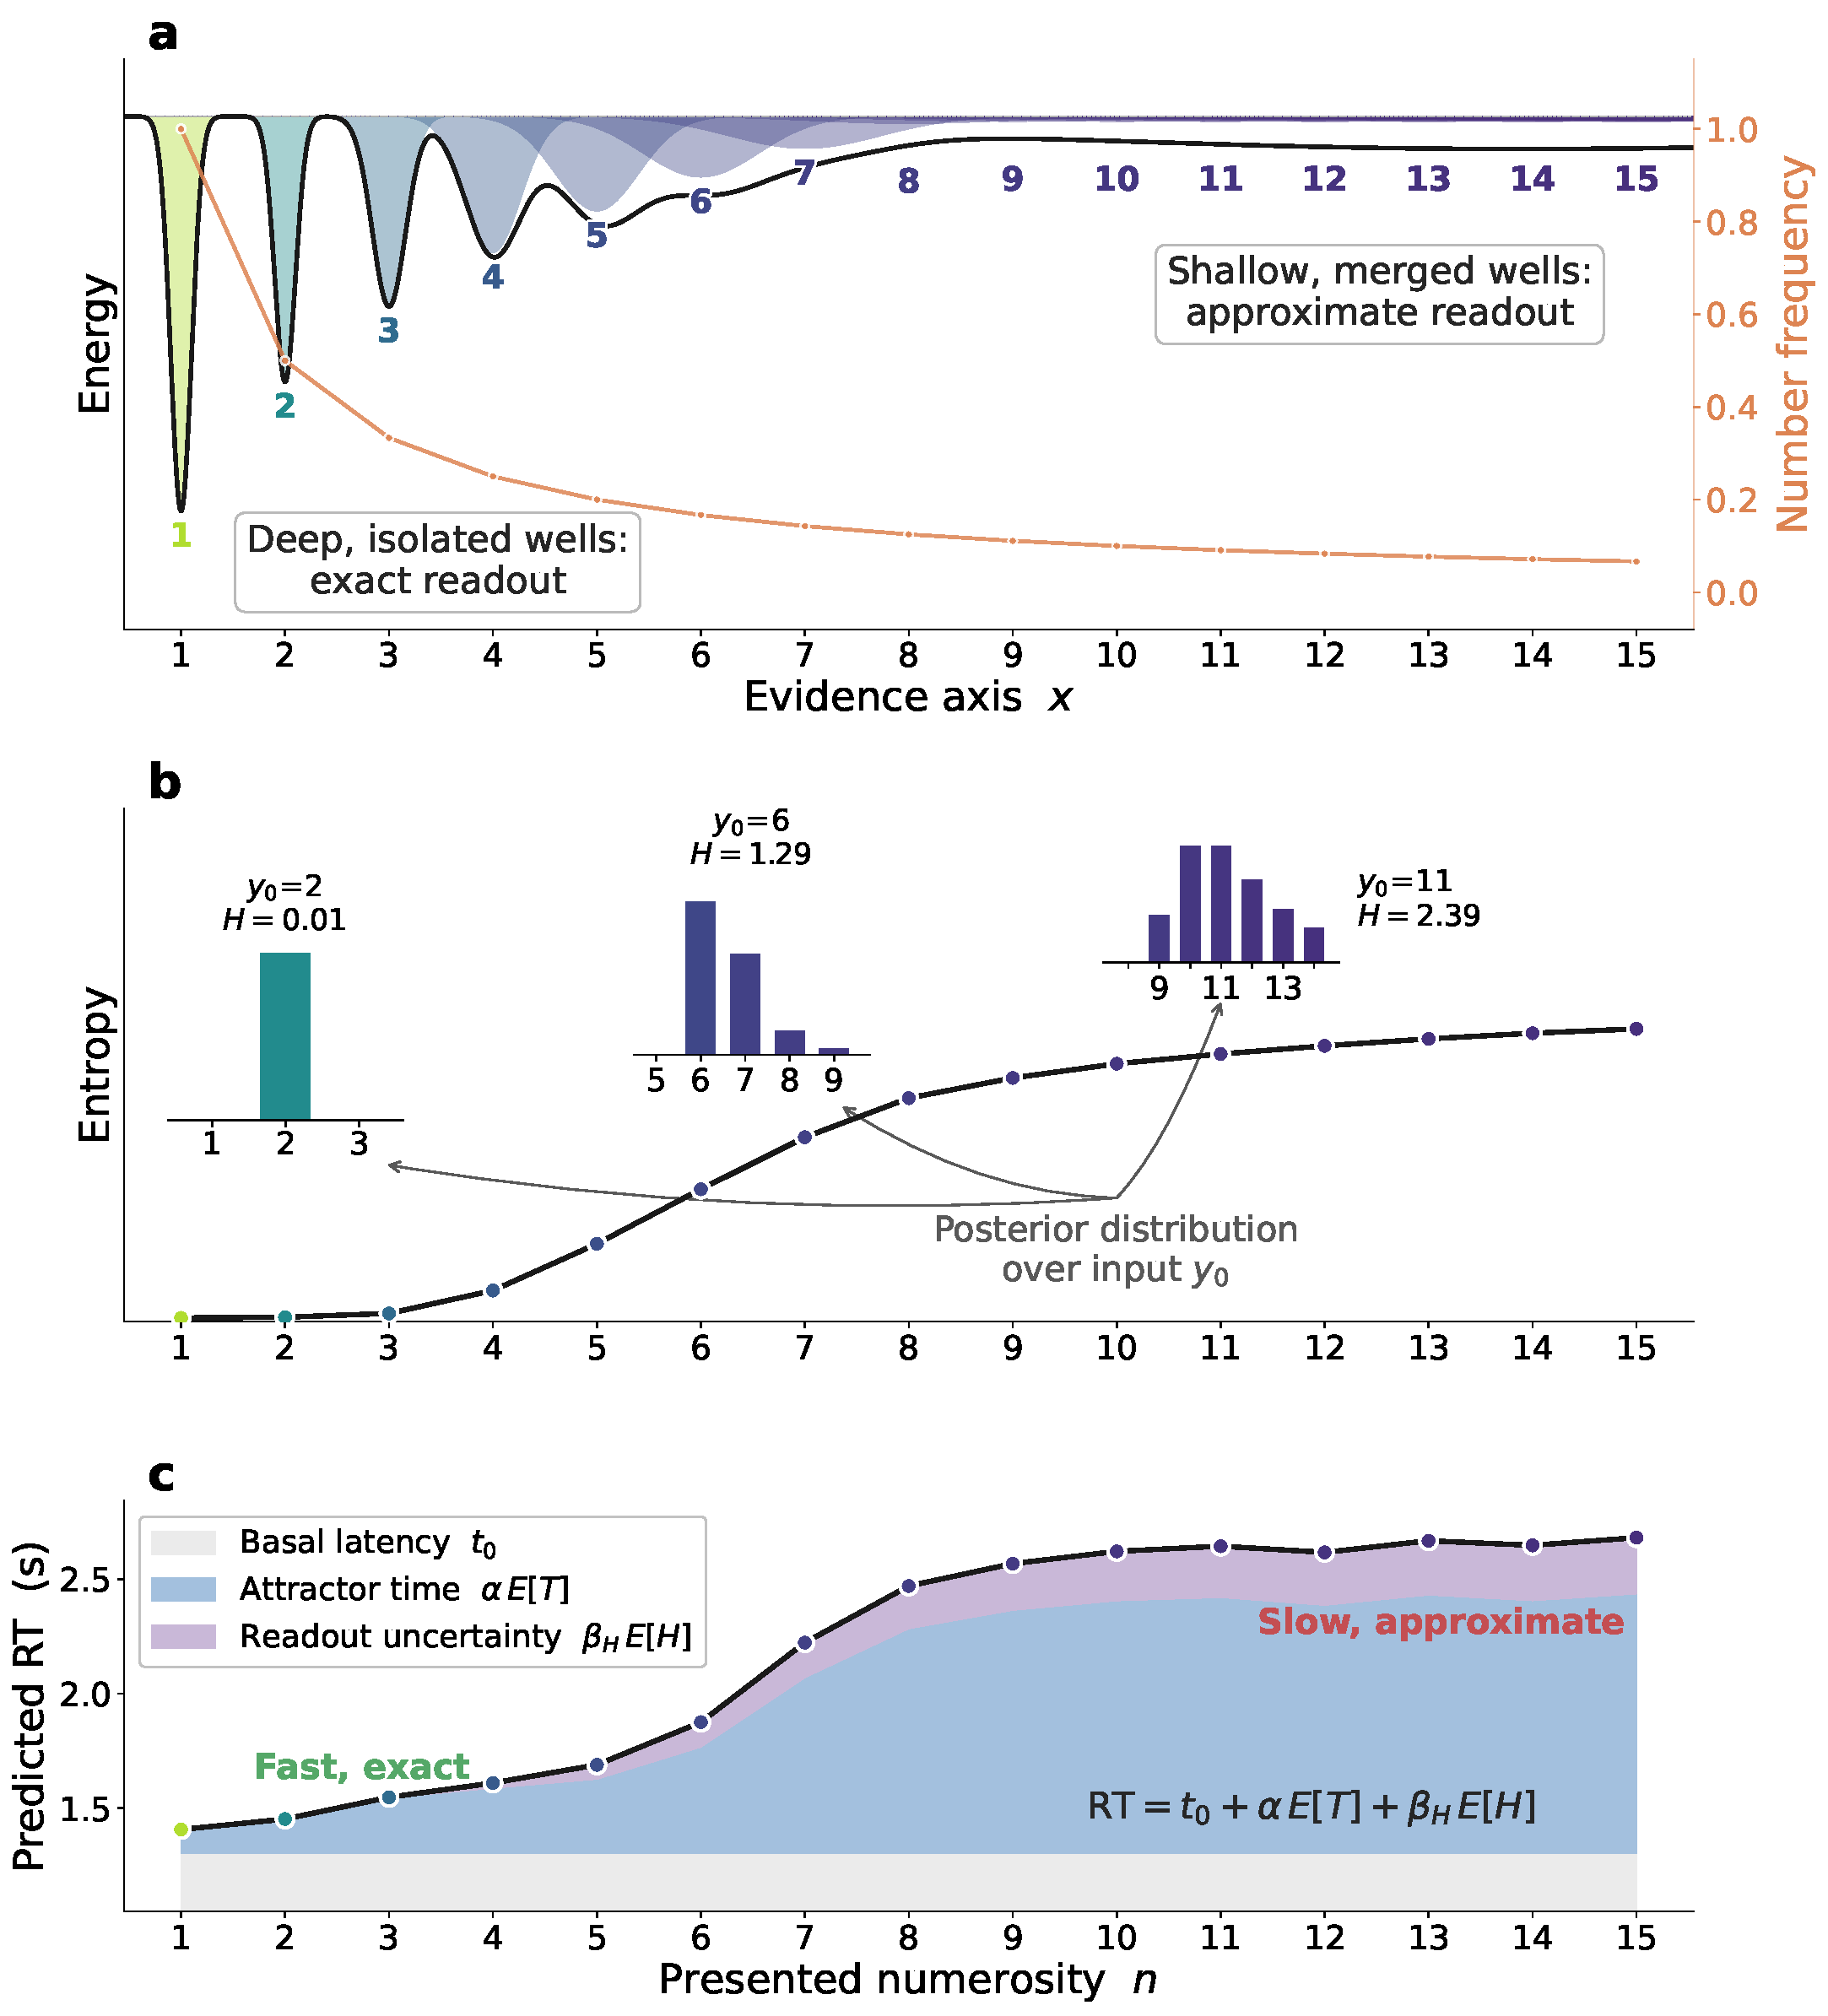
\includegraphics[width=\columnwidth]{../figures/conceptual_attractor_wells_ens.pdf}
  \caption{\textbf{The attractor model of the number line (parameters fitted at 160~ms).} \textbf{a}, Energy landscape over the internal evidence axis $x$: each integer is a well whose width grows with magnitude (the orange curve is the declining number frequency that motivates this widening), so small numbers sit in deep, isolated basins that clean up to an exact value. The dotted line marks the continuous width-based proxy $n_{\mathrm{width}}$, where $\sigma_n = 1$; the topological analysis in Fig.~\ref{fig:comparison}e directly determines where consecutive integer basins disappear. \textbf{b}, Expected readout entropy $E[H]$ per presented numerosity, before (grey) and after (black) clean-up, with the attractor's expected convergence time $E[T]$ (blue, right axis); insets show example post-clean-up posteriors. Clean-up removes the residual uncertainty of the small-$n$ readout at the cost of a few settling steps; near the boundary the settling time grows and the residual entropy rises. \textbf{c}, The resulting response time, $\mathrm{RT} = t_0 + \tau\,E[T] + \kappa\,E[H]$, decomposed into its basal, convergence-time, and readout-uncertainty components.}
  \label{fig:conceptual}
\end{figure}

In our landscape, each integer $n$ acts as a stored memory represented by a normalized Gaussian component centred at $n$. Its scale $\sigma_n$ controls both the breadth and the effective depth of the resulting basin: increasing $\sigma_n$ broadens the component and, through the normalization term $-\log\sigma_n$, lowers its peak contribution to the log-sum-exp landscape. We use the cross-linguistic power-law decline in number-word frequency~\citep{dehaene_cross-linguistic_1992} to motivate this coupled scaling, so frequent small numbers form narrow, deep basins and rarer large numbers form broad, shallow ones. Accordingly, the Gaussian scale grows as a power of magnitude,

%
\begin{equation}\label{eq:width}
\sigma_n = \sigma_{c}\, n^{p},
\end{equation}
%
where $\sigma_c$ sets the overall scale and the exponent $p$ controls how fast resolution degrades with magnitude. Each well contributes a log-likelihood
%
\begin{equation}\label{eq:well}
g_n(x) = -\log\sigma_n - \frac{(x - n)^2}{2\,\sigma_n^2}.
\end{equation}
%
Using the log-sum-exp energy form associated with modern Hopfield networks~\citep{ramsauer_hopfield_2021}, the attraction potential is the log-sum-exp over all wells, $V(x) = -\log \sum_n \exp\!\big(g_n(x)\big)$.

A sensory estimate $y_0 \sim \mathcal{N}\!\big(n,\; s_{00}^2 + s_{0}\,n^{\lambda_0}\big)$, whose noise grows with numerosity ($s_{00}$ fixed, $s_0$ and $\lambda_0$ fitted). From $x = y_0$ the state descends the potential, $x_{t+1} = x_t - \eta\,\partial V/\partial x$. Because $V$ is a log-sum-exp over the stored integers, each step moves the state toward a softmax combination of the wells, weighted by their precisions, so every stored integer contributes to the final position. The descent runs until the state settles or begins to oscillate, giving a resting state $x^*$ reached in $T$ steps. A distribution over integers is then read out, $p(n \mid x^*) = \mathrm{softmax}\!\big(g_n(x^*)\big)$, from which we take the mean estimate and the most probable integer.

The model gives a natural interpretation of response time as the combination of the time it takes for the clean-up mechanism to settle on a well, together with the uncertainty of the integer resolution, which we posit increases the decision time, and which is characterized by the entropy of the final state:
%
\begin{equation}\label{eq:rt}
\mathrm{RT} = t_{0} + \tau\,\mathbb{E}[T] + \kappa\,\mathbb{E}\big[H(p(n \mid x^*))\big],
\end{equation}
%
where $T$ is the number of clean-up steps, $H = -\sum_n p \log p$ is the residual readout entropy, and expectations are taken over the sensory noise. The convergence-time term $\tau\,\mathbb{E}[T]$ captures the deliberation the attractor dynamics require (long near the boundary, where the landscape flattens and the state settles slowly), while $\kappa\,\mathbb{E}[H]$ captures how undecided the readout remains between neighbouring integers. We compare this hybrid link against its two nested special cases (entropy only, $\tau=0$; steps only, $\kappa=0$). The basal latency $t_0$ is task-specific and fixed per dataset.

We fit the model to the individual responses of~\citet{cheyette_unified_2020}, in which adult participants ($N = 100$ per condition) briefly viewed dot arrays of $1$--$15$ items and typed an estimate, at five exposure durations (40, 80, 160, 320, 640~ms). We evaluate the categorical likelihood of the ${\sim}53{,}000$ individual integer reports. For each numerosity the response probability marginalises the readout over the sensory noise,
%
\begin{equation}\label{eq:marginal}
p(r \mid n) = \int p\big(r \mid x^*(y_0)\big)\,\phi\!\big(y_0; n, \sigma(n)\big)\,dy_0,
\end{equation}
%
computed by deterministic grid quadrature (\hyperref[sup-sm:methods]{Supplementary Material~1}). Typed responses run well beyond the well support, so we add a uniform lapse channel, $p_{\mathrm{final}}(r \mid n) = (1-\ell)\,p(r \mid n) + \ell\,/\,R_{\max}$, with $\ell$ fitted per duration and counted in all information criteria. The response model therefore has four mechanism parameters ($\sigma_c$, $s_0$, $\lambda_0$, $p$) plus the lapse, fitted by differential evolution~\citep{storn_differential_1997} and Nelder--Mead polishing both separately per duration and, as a stricter test, with the landscape shared across durations (\hyperref[sup-sm:comparison]{Supplementary Material~2}); the RT channel adds $\tau$ and $\kappa$. The response and response-time likelihoods are optimized as described in \hyperref[sup-sm:methods]{Supplementary Material~1}.

We fitted the model to the ${\sim}53{,}000$ individual responses in two ways. Our primary analysis used a joint fit in which a single power-law landscape ($\sigma_c$ and $p$) was shared across all five exposure durations, while the sensory channel and lapse were allowed to vary by duration. This directly tests whether one numerical representation can account for the full dataset. As a secondary, more flexible analysis, we fitted each duration separately to characterize condition-specific departures from the shared-landscape account. Both analyses were compared under the same trial-level likelihood against a graded set of alternatives. Matched static readouts isolate the contribution of clean-up for both width laws, whereas constant-width controls fix $p=0$ to isolate the contribution of magnitude-dependent broadening. A Weber/ANS code and the bounded-optimal model of~\citet{cheyette_unified_2020} benchmark the account as a whole. Parameter sharing, total model flexibility, and the corresponding AIC and BIC values are reported in Supplementary Table~S1.

We fitted the model to the ${\sim}53{,}000$ individual responses in two ways. Our primary analysis used a joint fit in which a single power-law landscape ($\sigma_c$ and $p$) was shared across all five exposure durations, while the sensory channel and lapse were allowed to vary by duration. This directly tests whether one numerical representation can account for the full dataset. As a secondary, more flexible analysis, we fitted each duration separately to characterise condition-specific departures from the shared-landscape account. Both analyses were compared under the same trial-level likelihood against a graded set of alternatives. Matched static readouts isolate the contribution of clean-up for both width laws, whereas constant-width controls fix $p=0$ to isolate the contribution of magnitude-dependent broadening. A Weber/ANS code and the bounded-optimal model of~\citet{cheyette_unified_2020} benchmark the account as a whole. Parameter sharing, total model flexibility, and the corresponding AIC and BIC values are reported in (\hyperref[sup-tab:model_comparison]{Supplementary Table~1}).

The landscape yields two complementary indices of numerical resolution. The continuous width-based index $n_{\mathrm{width}}$ is defined by $\sigma_n=1$, where the fitted Gaussian-component width equals the unit spacing between integers. With $\sigma_n=\sigma_c n^p$, this gives $n_{\mathrm{width}}=\sigma_c^{-1/p}$. The definition is equivalent to the heuristic $d'=\mathrm{spacing}/\sigma_n=1$~\citep{macmillan_detection_2004}, but it does not locate a topological merger. The topological index $n_{\mathrm{topo}}$ is computed directly from the fitted total potential $V(x)$. For each fit, we bracket all roots of $\partial V/\partial x$ on a dense grid, refine them numerically, classify the resulting minima and maxima, and assign each minimum to its nearest integer. We define $n_{\mathrm{topo}}$ as the largest consecutive integer from one that retains an assigned minimum separated from the preceding basin by an intervening energy maximum. Supplementary Material~4 gives the numerical details and grid-resolution check.

Finally, as an exploratory application, we fit the same model to the exact-enumeration data of~\citet{decarli_impaired_2020} from children with and without developmental dyscalculia, localizing the group difference within the landscape (\hyperref[sup-sm:dyscalculia]{Supplementary Material~5}).


%% ====================================================================
\section{Results}
%% ====================================================================

In the primary shared-landscape comparison, the attractor provided the best account of the trial-level responses (Fig.~\ref{fig:comparison}a; \hyperref[sup-sm:comparison]{Supplementary Material~2}). The constant-width attractor trailed by $\Delta\mathrm{AIC}\approx3405$, despite having one fewer parameter. The Weber/ANS code trailed by $\Delta\mathrm{AIC}\approx760$, despite retaining its full per-duration freedom, and the bounded-optimal model of~\citet{cheyette_unified_2020} trailed by approximately $11{,}400$ when given a matched duration-specific lapse. The same model ordering was recovered in the secondary duration-specific fits (Fig.~\ref{fig:comparison}b), where the constant-width ablation trailed by approximately $6600$. The corresponding differences for Weber/ANS and the bounded-optimal model were approximately $4300$ and $13{,}200$. The fitted width grows with magnitude, so the wells come out sharp and well-separated for small numbers and broad and overlapping for large ones; its scale and exponent trade off and are not interpreted singly, so we read the width law through the resolution limit it implies (\hyperref[sup-sm:recovery]{Supplementary Material~3}).

We also analyse the effect of the attractor dynamics in the model performance. If we switch them off, so that we have static readout of the same wells with the same number of parameters, the model fits worse by $\Delta\mathrm{AIC} \approx 640$ under the joint fit, and $\approx 1330$ with separate fits. This means that the dynamics sharpen the response distribution without adding fitted parameters. Nevertheless, as shown in Figure~\ref{fig:comparison}b, the static version of the model performs better at 320--640~ms. We postulate that this reflects the fact that, for these long exposures, the attractor has largely settled during the exposure itself, leaving little for the post-stimulus dynamics to resolve.

Because clean-up is a dynamical process, response time can be derived from how long it runs, not only from a static uncertainty proxy. The hybrid link that combines the attractor's convergence time with the residual readout entropy is the best account of RT (Fig.~\ref{fig:comparison}c,d), ahead of the residual-entropy proxy by $\Delta\mathrm{AIC} \approx 575$ with separate fits per duration and $\approx 850$ when a single RT mapping is shared across durations. Neither term suffices on its own: the two play complementary roles (Fig.~\ref{fig:conceptual}b--c), with the convergence-time term driving most of the rise in RT near the boundary, where the landscape flattens and the state settles slowly, and the residual-entropy term dominating once the wells have merged. Therefore, this model offers a second readout of the same fitted mechanism which accounts for the response times.

In the primary joint fit, the shared width law gives $n_{\mathrm{width}} = 8.3$, whereas direct analysis of the same potential gives $n_{\mathrm{topo}} = 6$ (Fig.~\ref{fig:comparison}e). The secondary duration-specific fits yield $n_{\mathrm{width}} \approx 3.5,\,6.7,\,8.3,\,9.1,\,9.8$ from 40 to 640~ms, while their topological limits are $n_{\mathrm{topo}} = 2,\,4,\,6,\,7,\,7$. Thus the continuous width proxy increases monotonically with viewing time, but the basin criterion is lower and plateaus after 320~ms. The response-time plateau occurs in a similar numerical region to the width-based values, but this descriptive alignment does not make $n_{\mathrm{width}}$ a behavioural or topological boundary (Fig.~\ref{fig:conceptual}c and Supplementary Fig.~\ref{sup-fig:rtdomain}). The two indices should therefore not be conflated: $n_{\mathrm{width}}$ summarizes the fitted width law, whereas $n_{\mathrm{topo}}$ identifies the last consecutive integer with its own basin.


\begin{figure}[t]
  \centering
  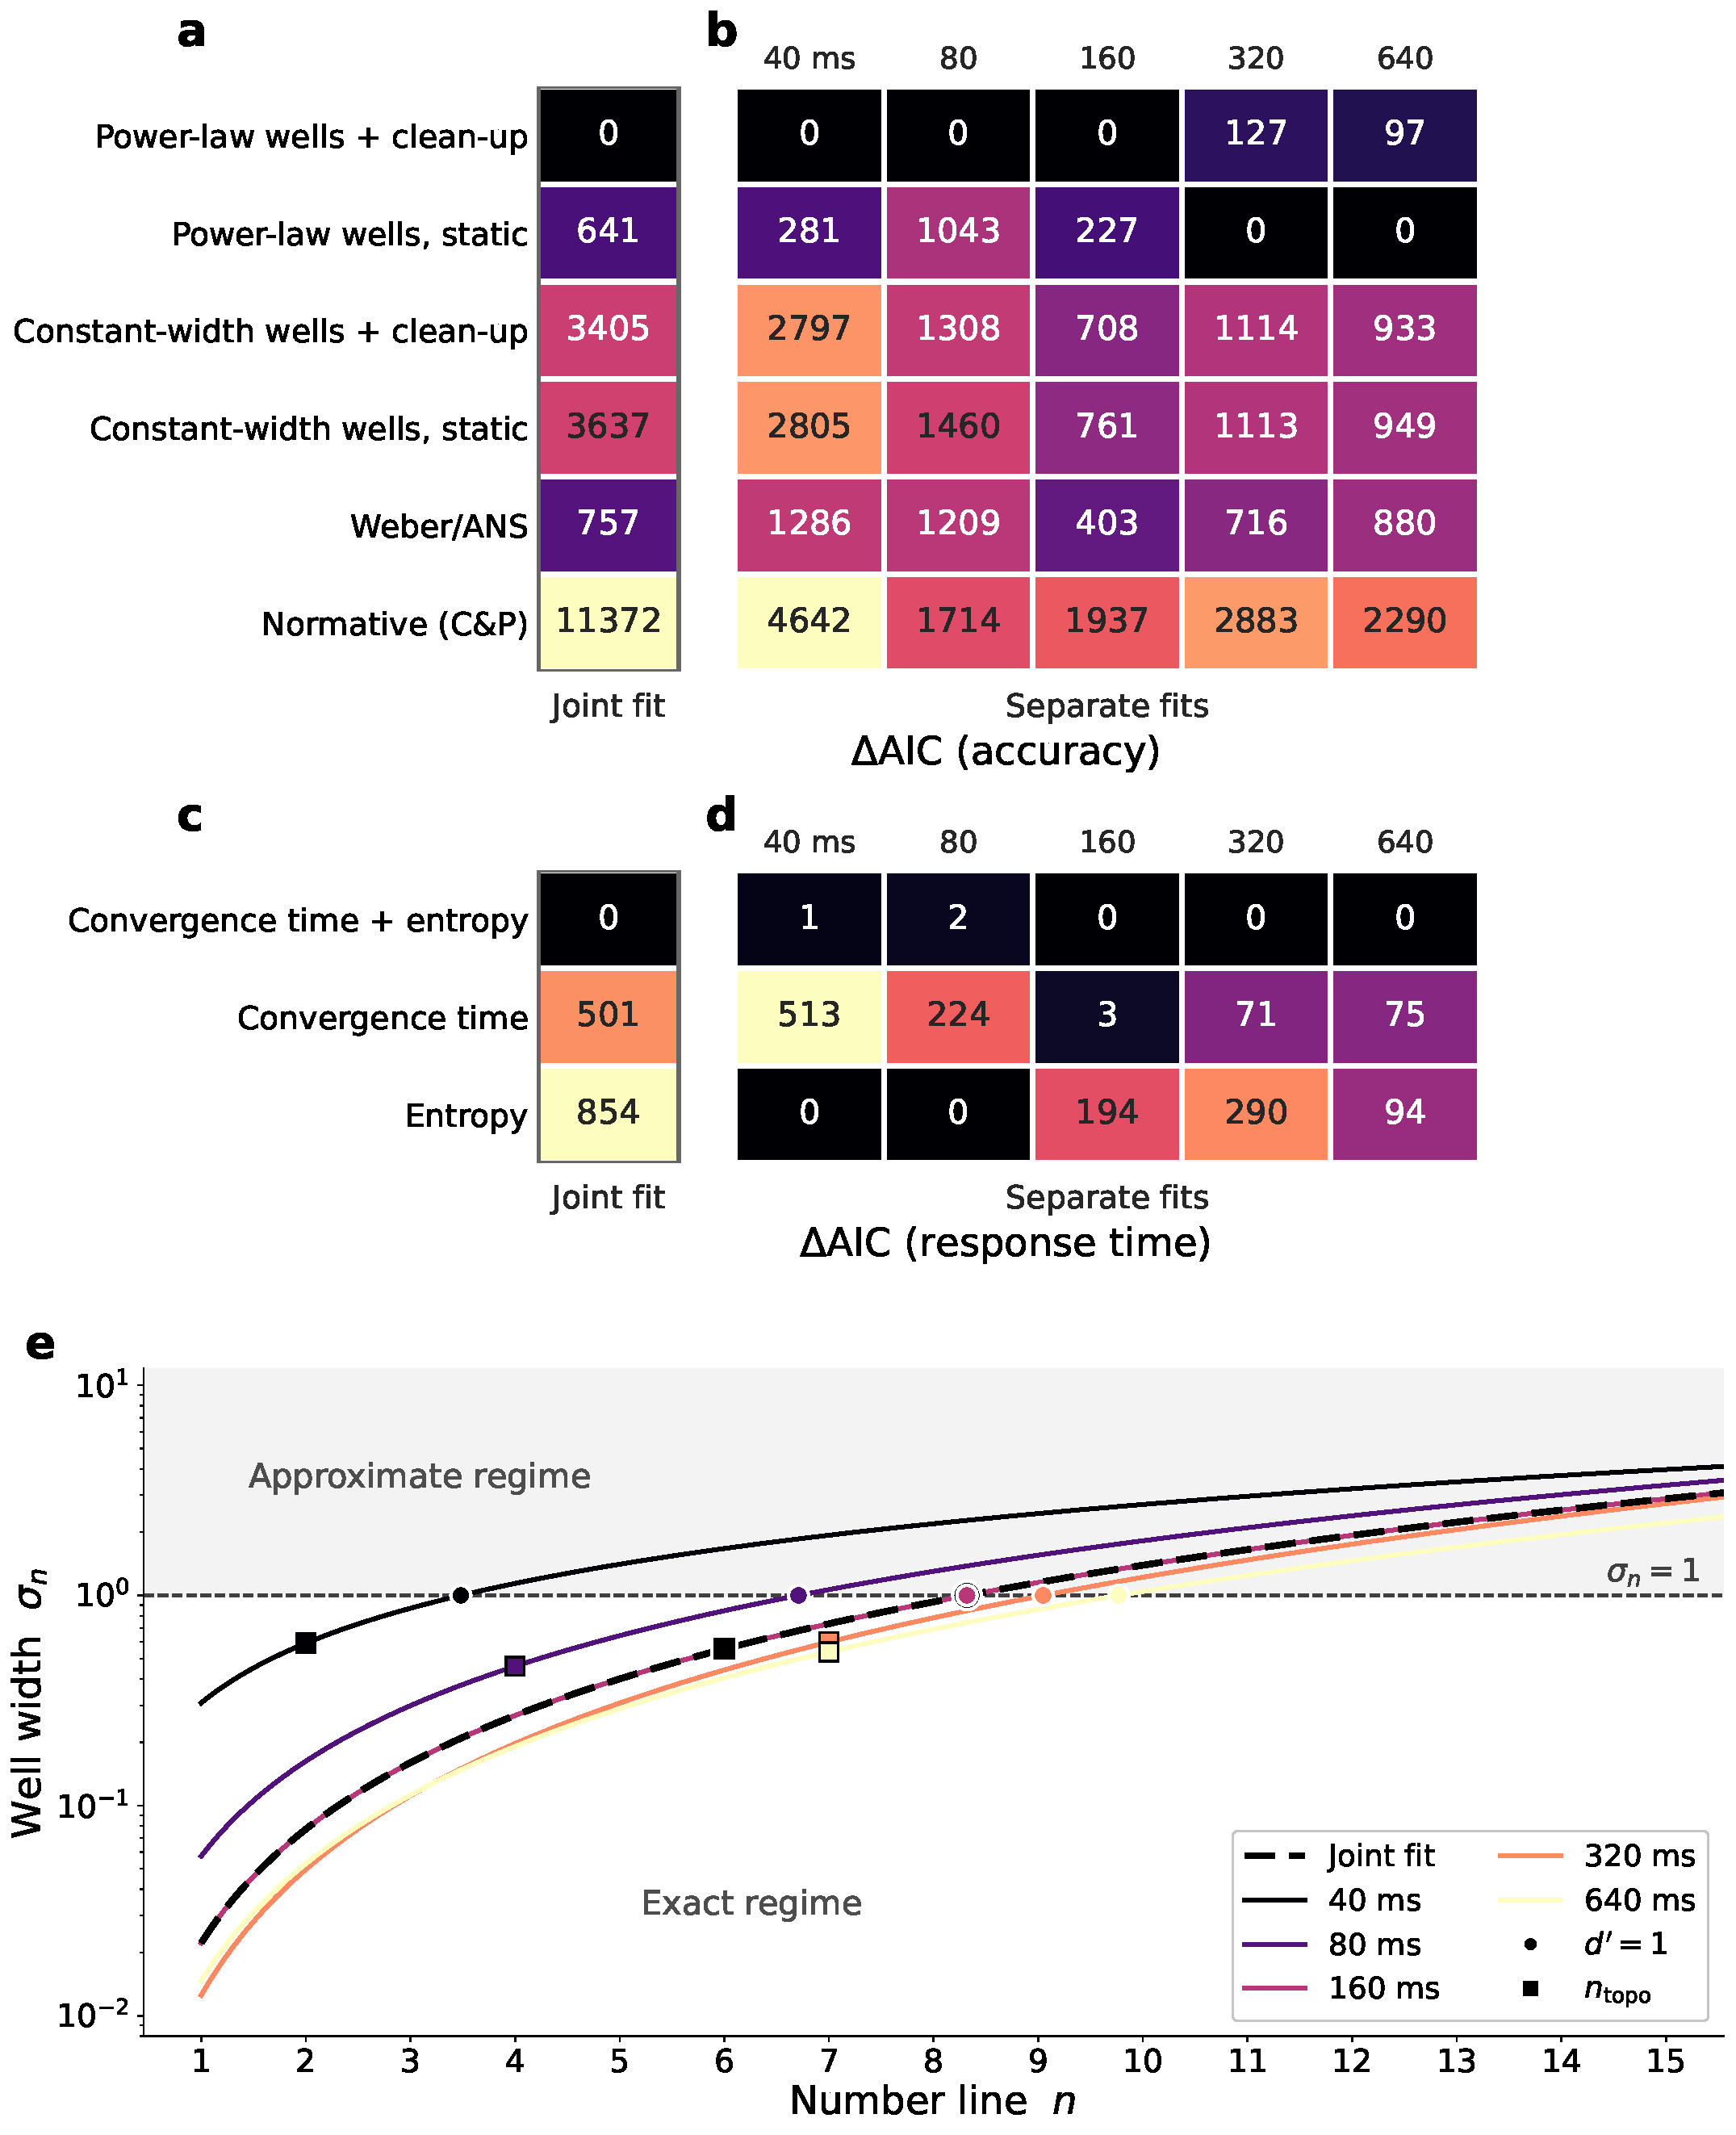
\includegraphics[width=\columnwidth]{../figures/fig3_comparison_ncrit.pdf}
  \caption{\textbf{Model comparison across exposure durations, response time, and the predicted resolution indices.} The model comparison is shown two ways: the primary joint fit, in which a single landscape is shared across all five durations, and the secondary separate fits per duration. \textbf{a}, Accuracy channel, joint fit: the power-law attractor and static readout share their landscape parameters ($\sigma_c$, $p$), while the constant-width controls fix $p=0$ and share only $\sigma_c$. Sensory parameters and lapse remain free per duration. Weber/ANS remains fully duration-specific. The bounded-optimal model of~\citet{cheyette_unified_2020} (``Normative (C\&P)'') shares $B$ and $R$ but uses a duration-specific lapse, matching the lapse flexibility of the other models. Cells are $\Delta$AIC relative to the best model (darker is better). \textbf{b}, Accuracy channel, separate fits per duration, over the ${\sim}53{,}000$ individual responses. The power-law wells ($\sigma_n = \sigma_c\,n^{p}$, Eq.~\eqref{eq:width}) and constant-width controls ($\sigma_n=\sigma_c$) each appear with clean-up and as a matched static readout. For C\&P, both the information budget and lapse are fitted per duration. Clean-up wins at the briefest exposures, while the static readout catches up at 320--640~ms. \textbf{c}, Response-time channel, joint fit: one RT mapping shared across durations. \textbf{d}, Response-time channel, separate fits on the winning landscape. In both, the link combining the attractor's convergence time and the residual readout entropy is best; neither term alone is sufficient, and their balance shifts across exposures. \textbf{e}, The fitted width law $\sigma_n$: the single shared landscape of the primary joint fit (black dashed) and the secondary per-duration fits (colours). Circles mark the continuous width-based index $n_{\mathrm{width}}$, defined by $\sigma_n=1$. Squares mark $n_{\mathrm{topo}}$, the last consecutive integer retaining its own local minimum separated by an energy barrier. The joint fit gives $n_{\mathrm{width}} \approx 8.3$ and $n_{\mathrm{topo}}=6$; the separate fits give $n_{\mathrm{width}}\approx3.5$--$9.8$ and $n_{\mathrm{topo}}=2$--$7$.}
  \label{fig:comparison}
\end{figure}

With these ingredients the model reproduces all three behavioural signatures together (Fig.~\ref{fig:fit}): pooled across durations, $R^2 = 0.99$ for the mean estimate, $0.92$ for exact accuracy, and $0.90$ for response time, the last obtained from a constrained cross-channel fit in which the landscape was held fixed at its response-fit values and only the RT mapping was estimated from response times. The one systematic miss is a mild under-prediction of exact accuracy in the ($n = 2$--$4$) band, most visible at the briefest 40~ms exposure: the model captures the trend toward near-perfect small-number performance but not its full sharpness, which we return to in the Discussion.

\begin{figure*}[t]
  \centering
  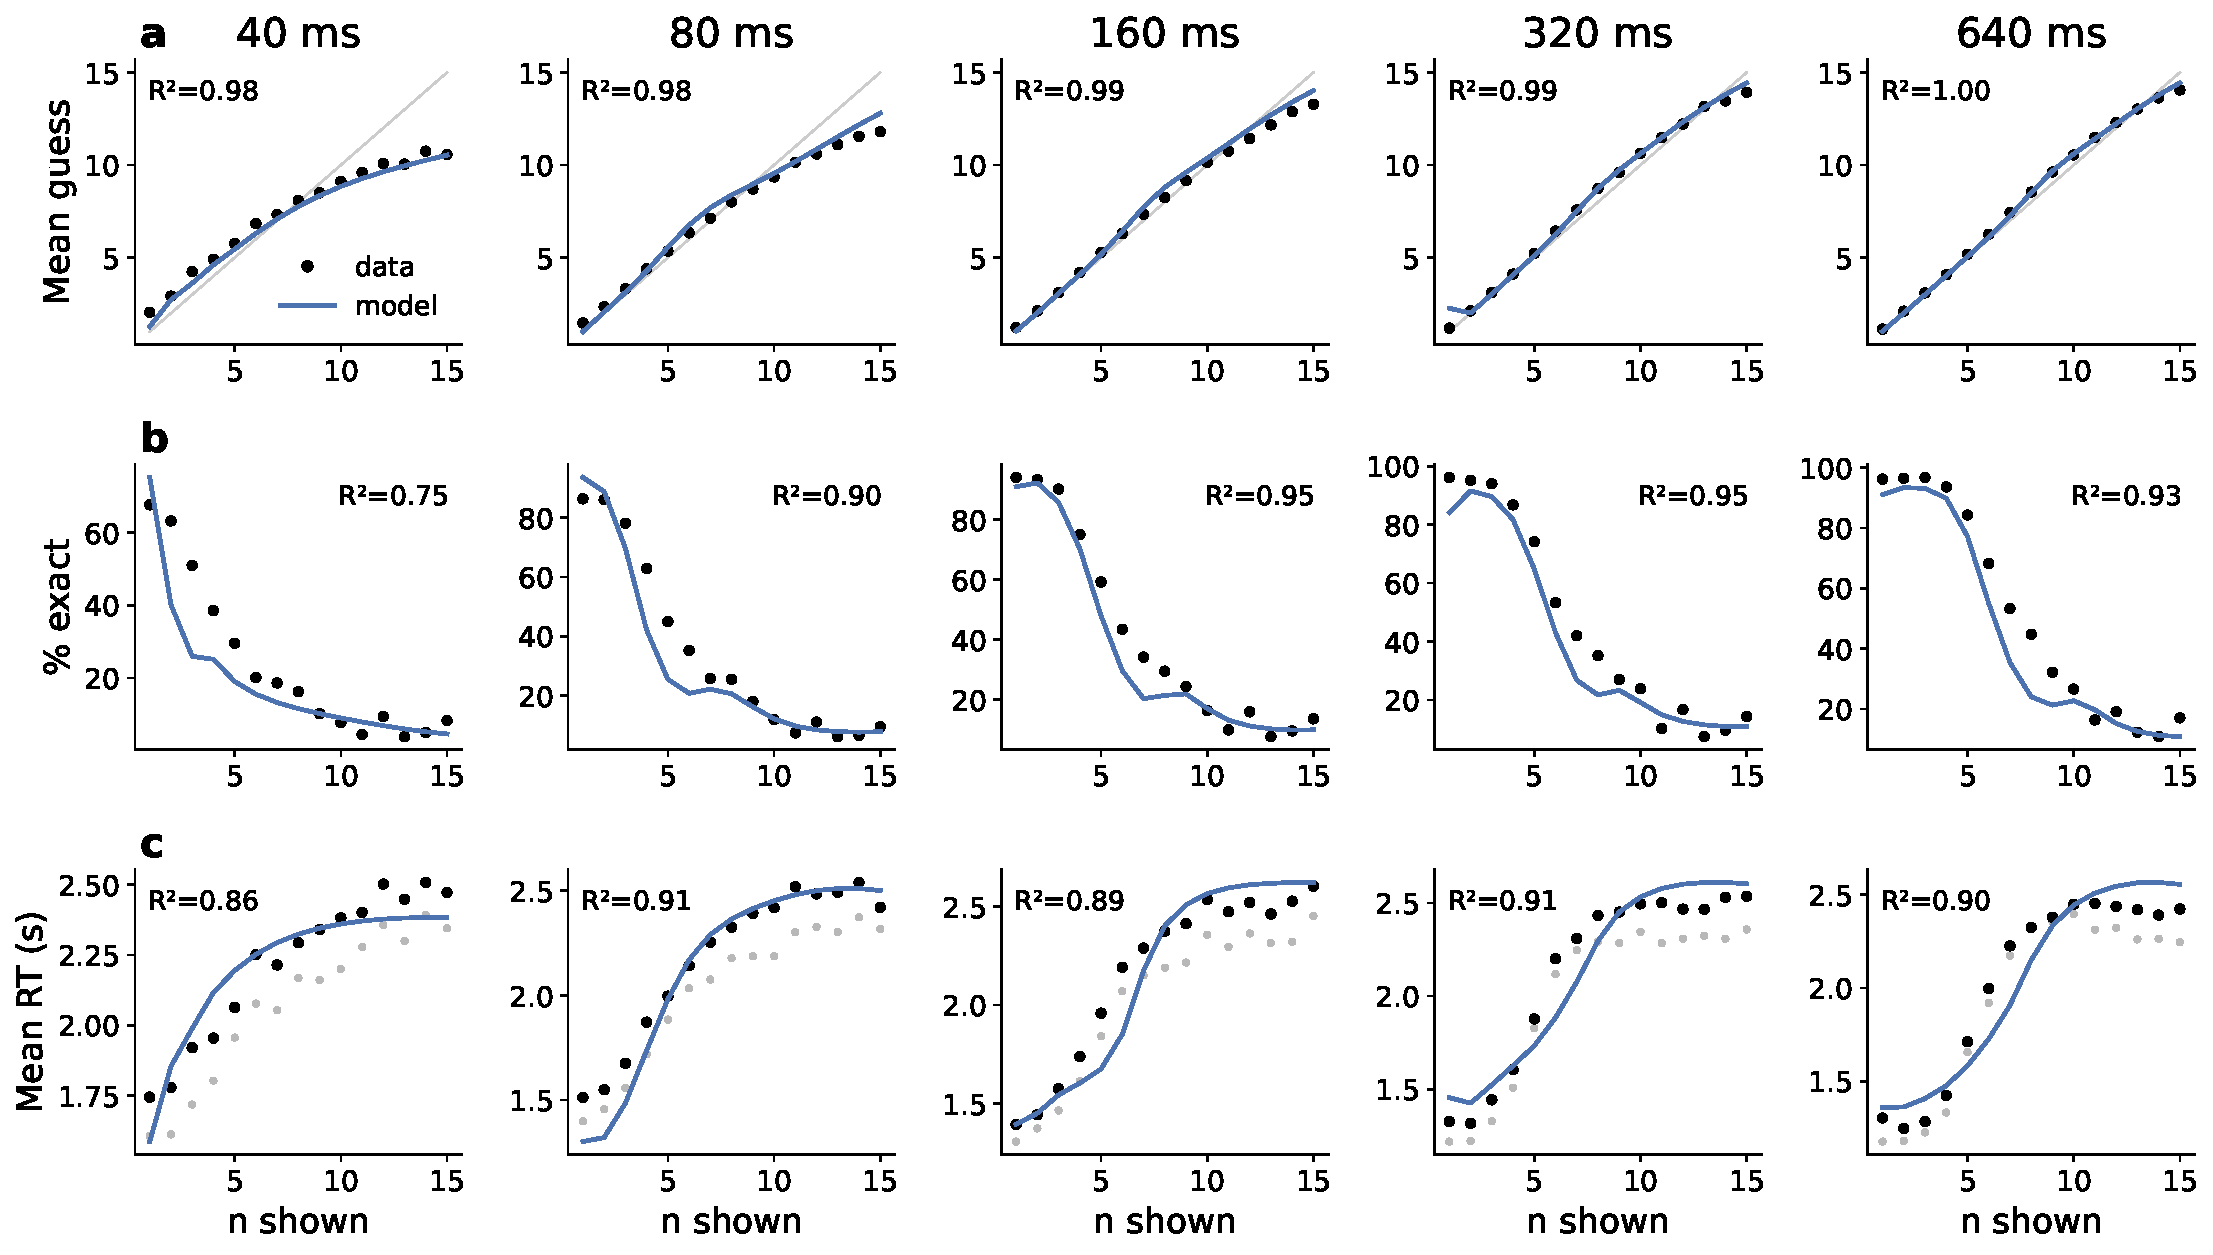
\includegraphics[width=\textwidth]{../output/trial_level_model_comparison/winner_fit_summaries.pdf}
  \caption{\textbf{Fit of the model to the~\citet{cheyette_unified_2020} data across the three channels.} Columns show presentation times from 40 to 640~ms; rows show the mean estimate, exact accuracy $P(r=n)$, and geometric-mean response time. Dots are empirical data (faint dots in the RT column are the median, shown for reference); lines are the model, with the landscape fitted to the individual responses. Response time is evaluated in a constrained cross-channel fit: the landscape is held fixed at its response-fit values, and only the RT-link parameters are fitted to the individual trial times. The small shoulder in predicted exact accuracy occurs near the width-based proxy $n_{\mathrm{width}}$ and disappears when clean-up is switched off (Supplementary Fig.~\ref{sup-fig:pexact}). $R^2$ values are given per panel.}
  \label{fig:fit}
\end{figure*}

A parameter-recovery analysis (\hyperref[sup-sm:recovery]{Supplementary Material~3}; Fig.~\ref{sup-fig:recovery}) confirms that the quantities we interpret are identifiable at the trial level: the width-based index $n_{\mathrm{width}}$ recovers in rank (Spearman $\rho = 0.98$) and the well width at $n=3$ accurately ($\sigma_3$, $R^2 = 0.89$), while the landscape's scale and exponent, like the two sensory parameters, trade off and are read only jointly through $n_{\mathrm{width}}$ and the noise profile $\sigma(n)$. A brief exploratory application to developmental dyscalculia reports the same width-based index in \hyperref[sup-sm:dyscalculia]{Supplementary Material~5} (Fig.~\ref{sup-fig:decarli}).

%% ====================================================================
\section{Discussion}
%% ====================================================================

We have described the inference of numerosity from noisy scalar evidence as pattern completion on an attractor landscape: the integers act like memories whose widths grow with magnitude, and an uncertain estimate relaxes toward the nearest resolvable region. Fitted to individual visual-enumeration responses, the model reproduces estimation, accuracy, and response time together and derives the loss of discrete resolution from the structure of the representation itself. The exact and approximate regimes become two readings of one numerical landscape rather than two systems joined at an unexplained seam.

Two features of the account carry the explanatory weight. The first is the clean-up dynamics. Turning clean-up on is a zero-parameter change, yet it improves the fit substantially, and the attractor's convergence time predicts response time better than a static uncertainty proxy. The clean-up implements a Hopfield-style associative retrieval operation: each step moves the state toward a softmax-weighted average of the stored integers, so every well shapes the outcome. Because those patterns are the ordered points of the number line, not arbitrary memories, the softmax competition among neighbours is sharp for small, well-separated numbers and broad for large, overlapping ones. The graded loss of resolution and the lengthening of settling time toward the boundary both follow from this structure. The second feature is that the wells broaden and become shallower with magnitude, mirroring the power-law decline of number frequency. This suggests a possible link between the geometry of the representation and numerical experience~\citep{anderson_reflections_1991, verguts_representation_2004}: frequent small numbers are sharply encoded, rare large ones diffusely.

If numerical experience shapes well width, development and training should progressively sharpen the fitted width profile. Both indices increase from 40 to 320~ms, but only $n_{\mathrm{width}}$ continues to increase at 640~ms; $n_{\mathrm{topo}}$ remains at seven. Exposure therefore changes the width profile without indefinitely extending the run of independent integer basins. Over development, we predict that numerical experience should alter both quantities, although whether basin topology continues to expand remains an empirical question. This change should be specific to exposure to \emph{numbers}, not to general visual acuity: an intervention that sharpens the number code should differ from one that improves perception at large~\citep{butterworth_investigating_2017}. The developmental dyscalculia analysis (\hyperref[sup-sm:dyscalculia]{Supplementary Material~5}) is an early step in this direction, although it currently estimates $n_{\mathrm{width}}$ rather than $n_{\mathrm{topo}}$.

The approximate regime is the same landscape read after the run of independent integer basins has ended. Beyond $n_{\mathrm{topo}}$, at least one consecutive integer no longer owns a distinct local minimum, and the readout becomes progressively coarser. At $n_{\mathrm{width}}$, the fitted component width reaches one unit; this statement concerns the width law, not the existence of an attractor. The model's response distributions match the data across the whole range, and their coefficient of variation settles to a roughly constant plateau at larger numerosities, matching the Weber fraction measured in numerosity estimation~\citep{testolin_estimates_2021} (Supplementary Fig.~\ref{sup-fig:weber}). One mechanism therefore accounts for exact and Weber-like approximate responses, but the change is gradual rather than a single shared boundary under both definitions.

The model's clearest failure is chronometric. The convergence-time term tracks response time over the lower-numerosity values but keeps rising where empirical RT plateaus (Fig.~\ref{fig:conceptual}c). Stratifying this mismatch around $n_{\mathrm{width}}$ is descriptive only. The model runs clean-up to convergence at every numerosity; participants appear instead to stop deliberating once the code is no longer useful for exact responding. Some mechanism halts the clean-up near the behavioural plateau and flattens response time, but the difference between $n_{\mathrm{topo}}$ and $n_{\mathrm{width}}$ shows that its trigger cannot be identified from either index alone. Because stopping early and running to convergence leave a similarly broad readout on overlapping wells, this affects latency more than the estimate. Whether numerosity adaptation involves the same halting is a natural question for future work.

This account complements visual accounts that explain how numerical evidence is constructed.~\citet{cheyette_limited_2024} derive number psychophysics from a bandwidth limit on visuospatial memory; in our model that limit would live in the sensory channel $\sigma(n)$, upstream of the attractor. The increase in $n_{\mathrm{width}}$ with exposure indicates a sharper fitted width profile, while the plateau in $n_{\mathrm{topo}}$ shows that this need not add another independent basin. Both accounts are shaped by the same empirical regularity, the power-law decline of number frequency with magnitude, though in our account it shapes well width rather than acting only as a prior over numerosity. The present account also posits a trainable attractor memory shared by any channel capable of supplying scalar numerosity evidence. Unlike recurrent accounts with fixed range partitions~\citep{sengupta_visual_2014}, its width-based and topological indices can vary separately, providing a more specific developmental prediction.

FALTA: dir alguna cosa sobre malo (maloquantum2023).

The present implementation isolates this recurrent numerical stage in two ways. First, the visual front end is summarised by a noise profile $\sigma(n)$, leaving the contribution of continuous image statistics such as area, density, and convex hull outside the model. Coupling the landscape to an image-computable front end that is itself sensitive to number~\citep{stoianov_emergence_2012, testolin_visual_2020}, and that has been used to simulate dyscalculic profiles~\citep{dolfi_weaker_2024}, would connect sensory encoding to the attractor dynamics. Second, the landscape is initialised with an already accumulated estimate $y_0$. A natural extension is a driven attractor in which evidence enters continuously as it becomes available. Sequentially registered dots, sounds, or touches could then move the state through the number line while recurrent clean-up stabilises the emerging estimate. This would connect evidence accumulation and associative retrieval within a single dynamical process and provide a direct cross-modal test of the proposed shared code.


The model also under-predicts the sharpness of small-number accuracy at $n=2$--$4$: it captures the trend but not the full abruptness of the subitizing edge, which may still require a fast, capacity-limited object-individuation process~\citep{feigenson_representations_2002, piazza_subitizing_2011}. Together with evidence for approximate-magnitude signatures in the small-number range~\citep{cordes_variability_2001}, this pattern suggests partially overlapping contributions of estimation and individuation within the subitizing regime~\citep{burr_subitizing_2010, mou_two_2014, briggs_attentional_2023}. Finally, the model is specified at a computational and algorithmic level; relating the wells to the number-tuned populations of parietal cortex, whose tuning widths grow with preferred numerosity~\citep{piazza_tuning_2004,harvey_topographic_2013}, is a natural direction for testing it neurally.

% a complementary line of functional neuroimaging work suggests encoding of individual objects may occur within the IPS as well (Culham et al., 1998, 2001; Xu and Chun, 2006; Xu, 2009). More specifically, recent work suggests that inferior IPS activity scales with the number of objects in scene up to about three to four and then plateaus while the superior IPS responds to differences in object identity, but not number. These results suggest that portions of the inferior IPS support the initial selection and individuation of a limited number of objects from a scene (up to about four), in contrast to the lateral occipital complex and the superior IPS, which seem to support object identification (Xu and Chun, 2006; Xu, 2009).

Numerical cognition, in this framework, is pattern completion on a landscape of number memories. A single set of wells, read exactly where they are resolved and approximately where they merge, accounts for the fast exactness of small numbers, the graded approximation of larger ones, the response times of both, and the moving boundary between them. The result is a compact, mechanistic set of hypotheses about how the mind represents number.

\begin{acks}
The author thanks Brian Butterworth, Diana Laurillard, and Marc Colomer for their comments and feedback, and the reviewers, whose detailed and constructive reviews substantially improved this manuscript.
\end{acks}

\section*{Author Contributions}
Eudald Correig-Fraga: Conceptualization, methodology, software, formal analysis, investigation, data curation, visualization, writing - original draft, and writing - review and editing.

\section*{Ethical Considerations}
This article reports computational modelling and secondary analysis of previously published, publicly available datasets. No new human participants were recruited, and no new human data were collected for this study. Ethical approval for the original data collections was reported in the source publications.

\section*{Consent to Participate}
Not applicable. This study did not recruit participants or collect new participant data.

\section*{Consent for Publication}
Not applicable. This study does not contain identifiable individual participant information.

\begin{funding}
This work was funded by Innovamat Education SL.
\end{funding}

\begin{dci}
The author declared no potential conflicts of interest.
\end{dci}

\section*{Data Availability}
Code is available at \url{https://github.com/eudaldc/hopfield_numbers}. The source datasets are available at \url{https://osf.io/svcy5/} and \url{https://osf.io/gjpb3/}.

\begin{sm}
Supplementary material is available with this article.
\end{sm}

% Harvard (author--year):
\bibliographystyle{SageH}
\bibliography{references}

\end{document}
